\documentclass{article}
\usepackage{stmaryrd}
\usepackage{graphicx}

\title{Report, Kinetic project}
\author{Dorian Geraldes Pereira, Axel Demuth}
\date{March 2024}

\begin{document}
\maketitle
\tableofcontents
\newpage


\section{Objectives}
To be able to solve equations on a mesh, we need it to be watertight.
\newline The objectives of the project are:
\newline
\begin{itemize}
    \item Repair mesh to make them watertight
    \newline
    \begin{itemize}
        \item watertight building model
        \newline
        \item watertight urban model
    \end{itemize} 
\end{itemize} 

In our project we will have to use files in IFC format containing building meshes that are not watertight in an algorithm repairing
geometric error in a kinetic data structures. We will have to find a way to keep the label 
on the surfaces in the algorithm or relabel every surfaces at the end.
we can see here an example of what we will need to do:\newline
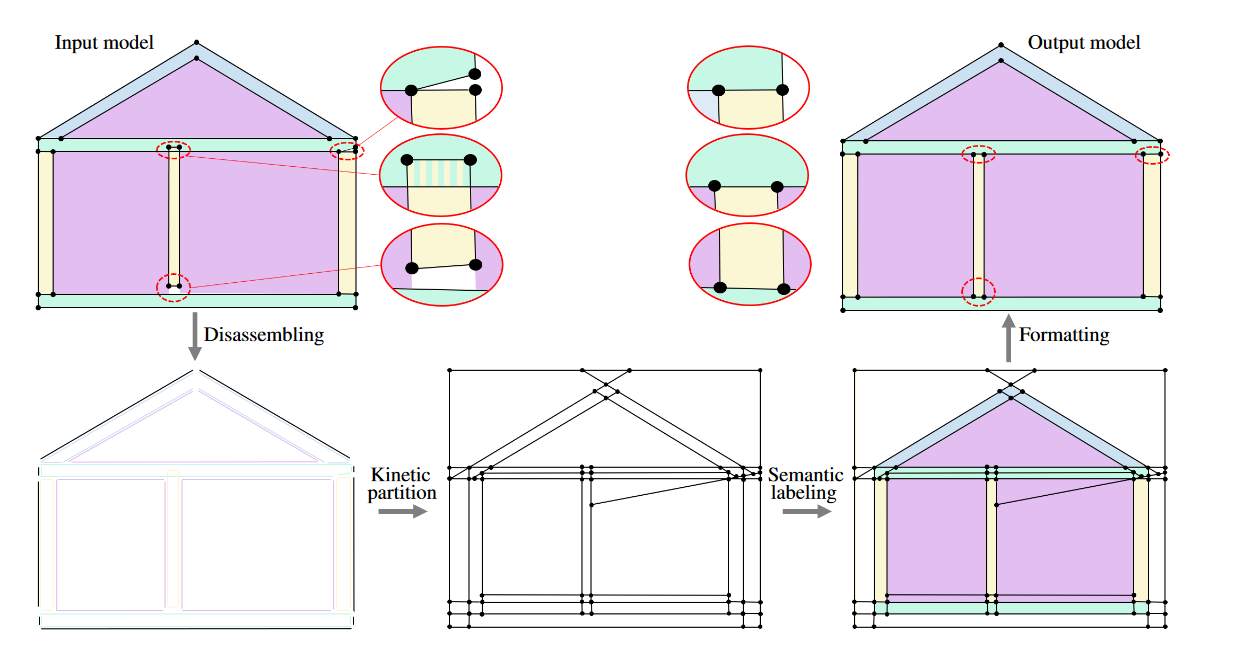
\includegraphics[scale = 0.37]{../../images/example_algorithm_2.png}



\section{Tools}
\subsection{CGAL}
CGAL is a comprehensive package for geometry algorithms, providing various data structures and algorithms for working on polygons, surfaces, mesh generation, and more.
It offers a wide range of functionalities for geometric processing and analysis in various fields such as computer graphics, computational geometry, and geometric modeling.
\subsection{Kinetic}

Kinetic algorithms is a package from CGAL that allows working on meshes with some holes in them. When applied to the mesh, the Kinetic algorithms will 'extend' some surfaces to fill the mesh and make it watertight. 
Here's what the algorithm is capable of:


\begin{figure}[h]
    
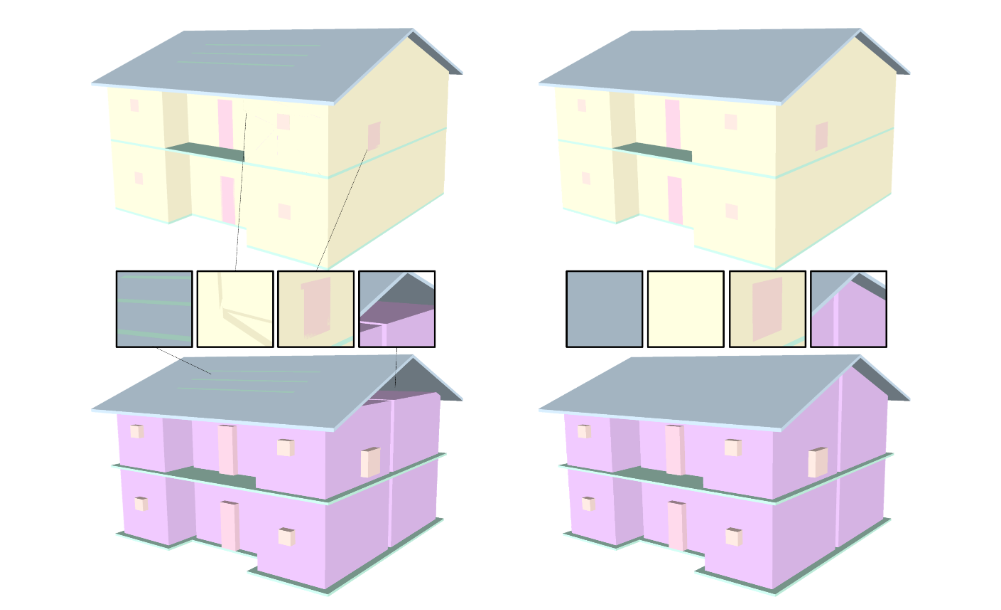
\includegraphics[scale =   0.3 ]{../../images/example_algorithm.png}

\end{figure}
\subsection{Roadmap}
We intend to work on this project in the coming months and will continuously update our progress as outlined in the following roadmap.
\begin{figure}[h]
    
    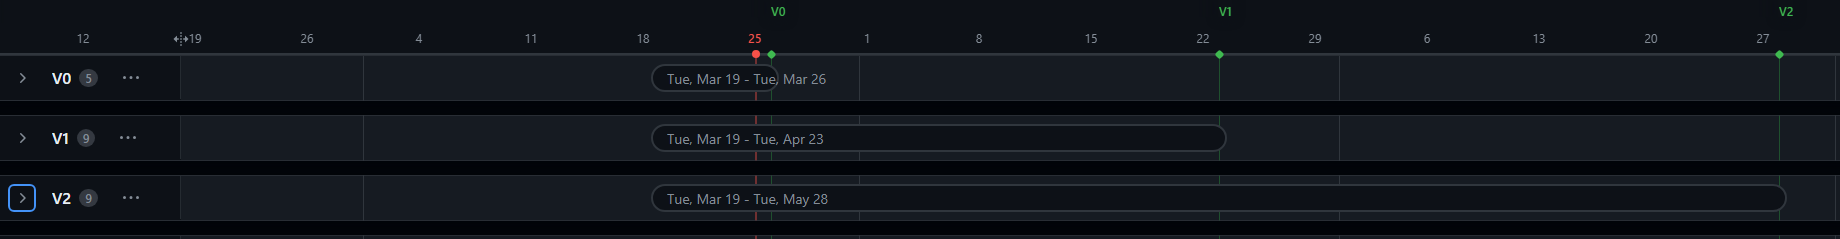
\includegraphics[scale =   0.3 ]{../../images/roadmap.png}
    \end{figure}
    
\nocite{*}
\bibliographystyle{plain}
\bibliography{../../bibliography/v0/report_bib}
\end{document}